\section{Theory}

\subsection{Reinforcement Learning}
    \subsubsection{The Reinforcement Learning Problem Setting}
    \subsubsection{Value-Based and Policy-Based Methods}
    \subsubsection{Policy Gradient Methods}

\subsection{Artificial Neural Networks}

\subsection{Electric Motor Dynamics}
    \subsubsection{Motor Modeling}
    \subsubsection{Torque Speed Models}

\subsection{Spring-Damper Systems}

\subsection{Kinematics, Jacobians, and Virtual Work}
    \subsubsection{Robot Kinematics}
    \label{sec:robot_kinematics}
Consider a robotic link arm existing in $\mathbb{R}^2$ consisting of $n$ links, each with a length $l_i$ and a joint angle $q_i$. The position of the end-effector is given by the vector $\mathbf{x} = [x, y]^T$, where $x$ and $y$ are the coordinates of the end-effector in the global coordinate system. Using simple trigonometry, the position of the end-effector can be expressed as a function of the joint angles and link lengths as seen in equation \ref{eq:robot_kinematics}. 
Axes and joint angles corresponding to the expression in equation \ref{eq:robot_kinematics} can be seen in figure \ref{fig:robotic_link_arm}. 

\begin{equation}
    \label{eq:robot_kinematics}
    \mathbf{x} = \begin{bmatrix}
        x \\
        y
    \end{bmatrix} = \begin{bmatrix}
        \sum_{i=1}^{n} l_i \cos(q_i) \\
        \sum_{i=1}^{n} l_i \sin(q_i)
    \end{bmatrix}
\end{equation}

\begin{figure}[H]
    \centering
    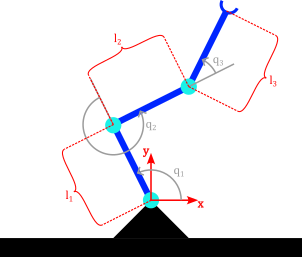
\includegraphics[width=0.5\textwidth]{Images/manipulator_inkscape_Layer 1.png}
    \caption{Illustration of a 3 link robotic link arm in $\mathbb{R}^2$ with $n$ links.}
    \label{fig:robotic_link_arm}
\end{figure}


    \subsubsection{Jacobian Matrix}

As described in section \ref{sec:robot_kinematics}, the position of the end-effector can be expressed as a function of the joint angles and link lengths. In robotics, it is often useful to express the relationship between infinitesimal changes in the joint angles and the resulting change in the end-effector position. As can be seen in equation \ref{eq:infinitesimal_change}, infinitesimal changes in variables $\delta y$ and $\delta x$ can be described by means of the partial derivative \cite{modsim}. If this is compared to the definition of the jacobian in equation \ref{eq:jacobian}, it is clear that the jacobian matrix $\mathbf{J}$ can be used to map infinitesimal changes in joint angles to changes in the end-effector position, as illustrated in equation \ref{eq:jacobian_pos_mapping}. The limit of an infinitesimal change over an infinitesimal time interval is a derivative, and thus by dividing each side in equation \ref{eq:jacobian_pos_mapping} by $\delta t$, one arrives at the expression in equation \ref{eq:jacobian_speed_mapping}, by which the jacobian can be used to map joint velocities to end-effector velocities.

\begin{equation}
    \label{eq:infinitesimal_change}
    \delta  y = \frac{\partial y}{\partial x} \delta x
\end{equation}

\begin{equation}
    \label{eq:jacobian}
    \mathbf{J} = \begin{bmatrix}
        \frac{\partial x}{\partial q_1} & \frac{\partial x}{\partial q_2} & \cdots & \frac{\partial x}{\partial q_n} \\
        \frac{\partial y}{\partial q_1} & \frac{\partial y}{\partial q_2} & \cdots & \frac{\partial y}{\partial q_n}
    \end{bmatrix}
\end{equation}

\begin{equation}
    \label{eq:jacobian_pos_mapping}
    \mathbf{\delta x} = \mathbf{J}\mathbf{\delta q}
\end{equation}

\begin{equation}
    \label{eq:jacobian_speed_mapping}
    \mathbf{\dot x} = \mathbf{J}\mathbf{\dot q}
\end{equation}

    \subsubsection{Force/Torque Mapping}

    Finally found northwestern book that says what I need: \cite{NorthWestern_Robotics}. 

    Consider a robotic manipulator with $n$ joints, each with a joint angle $q_i$ and a joint torque $\tau_i$. The position of the end effector for such a system is given by equation \ref{eq:robot_kinematics}, and thus the formula in equation \ref{eq:jacobian_speed_mapping} can be used to map joint velocities to end effector velocities. 

    


\subsection{Dynamical Systems and Contact Dynamics}
    \subsubsection{Rigid-Body Dynamics}
    \subsubsection{Contact Modeling and Impact Dynamics}
    \subsubsection{Friction Models}
